\chapter{Exploration of atomistic predictions}






\section{ANAKIN-ME predictions}
Here I should be writing about the ANI predictions in greater detail than the background information

Add content from pages 5-15 of qualifying exam document -- will need significant rewriting, but the details of the work completed there is useful for filling this section in. 
\subsection{Total energy as a sum of atomic energies}

\subsection{Uncertainty in ANI neural network potentials}

\subsection{Exploration of the flaws in predicting total energy as a sum of atomic energies}

\typeout{Graphic file (Images/CH4.png) not found!}

\begin{figure}[!hb]
    \centering
    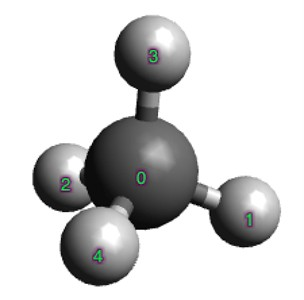
\includegraphics[width=3in]{Images/CH4.jpg}
    \caption{I don't know why this image doesn't show up.}
    \label{ch4}
\end{figure}{}

% Tables suck, but this helped me align columns and headers separately:
\begin{table}[!hb]
\centering
\caption{
Atomic energy contributions by atom type in a geometry-optimized molecule of CH\textsubscript{4}, with four equivalent hydrogen atoms. 
Additionally, the sum over all atoms, and that sum after passing through the TorchANI EnergyShifter. 
Values obtained from an ensemble of ANI models (ANI-DR); the last column shows the standard deviation of predictions across the ensemble. 
All values are in kcal/mol.
}\label{ch4_AEs}
    \begin{tabularx}{\textwidth}{%
    >{\raggedleft\arraybackslash}r  % Numeric
    >{\raggedleft\arraybackslash}r  % Numeric
    >{\raggedleft\arraybackslash}r  % Numeric
    >{\raggedleft\arraybackslash}r  % Numeric
    >{\raggedleft\arraybackslash}r  % Numeric
    }  
      \hline
      Model & Carbon & Hydrogen & Sum of atomic energies & Molecular energy \\
      \hline
      1 & -4.467 & -1.834 & -11.803 & -25413.871 \\
      2 & 15.049 & -6.709 & -11.787 & -25413.855 \\
      3 & 1.656 & -3.352 & -11.754 & -25413.822 \\
      4 & -8.199 & -0.882 & -11.728 & -25413.796 \\
      5 & -7.859 & -0.958 & -11.691 & -25413.759 \\
      6 & 6.757 & -4.636 & -11.787 & -25413.856 \\
      7 & -1.683 & -2.492 & -11.652 & -25413.720 \\
      8 & -4.101 & -1.824 & -11.395 & -25413.463 \\
      Standard deviation & 7.437 & 1.871 & 0.125 & 0.125 \\
      \hline
    \end{tabularx}
\end{table}


\section{Drawback of atomic energy predictions}

insert images of hydrogen / carbon / nitrogen / oxygen stdev histograms, 

\section{Need for a practical, physical quantity to estimate uncertainty}

Looking for a correlation between the energy error and the predictive uncertainty of a given \textbf{atomic} quantity.
